\chapter{Non-Negative Matrix Factorization}
In this chapter the formulation of the Non-negative matrix factorization (NMF) problem is presented along with the main results that characterize it.
\par
In section \ref{Metrics section} the most common metrics used in the NMF literature are discussed, specifically the Frobenius norm \ref{Frobenius norm section}, the Kullback-Leibler divergence \ref{Kullback-Leibler section}, and the $\beta$-divergence \ref{Beta divergence section}.
In section \ref{complexity of NMF section} the main result on the computational complexity of NMF is presented, namely that this problem is NP-hard in general \cite{vavasis2007complexitynonnegativematrixfactorization}.
Section \ref{Non-negative rank section} contains the important definition of the non-negative rank of a non-negative matrix.
Then, section \ref{identifiability section} discusses the identifiability problem of NMF, that is the non-uniqueness of the solutions of the NMF problem in general.
Section \ref{Geometric interpretation section} concerns the geometric interpretation of NMF, in particular a linear dimensionality reduction perspective is given along with a brief overview of the geometric interpretation with cones.
Finally in \ref{two applications of NMF section} two applications of NMF are presented: feature extraction from a dataset of grey scale faces images \ref{Example feature extraction NMF} and topic modeling from a collection of documents \ref{Topic modeling section}.
\section{Definition}
In its more general form the Non-negative matrix factorization problem can be defined as follows: given a non-negative matrix $V \in \R_+^{m \times n}$ and a factorization rank $r \in \N$ find two matrices
$W \in \R_+^{m \times r}$ and $H \in \R_+^{r \times n}$, constrained to be non-negative, such that their product $WH$ approximates $V$ as closely as possible according to some distance measure $D$.
\par
This problem can be formulated with an optimization problem as follows:
\begin{definition}[Non-Negative Matrix Factorization optimization problem]\label{NMF optimization problem}
Given a non-negative matrix $V \in \R_+^{m \times n}$ and a factorization rank $r \in \N$, find two non-negative matrices $W \in \R_+^{m \times r}$ and $H \in \R_+^{r \times n}$ that minimize 
a given cost function $D(V, WH)$, that is:
\begin{equation}
\min_{W \in \R_+^{m \times r}, H \in \R_+^{r \times n}} D(V, WH)
\end{equation}
where $D$ is a distance measure between matrices.
\end{definition}
\begin{remark}
    $\R_+^{m \times n}$ denotes the set of all $m \times n$ matrices with non-negative entries, the problem \ref{NMF optimization problem} is a constrained optimization problem where the optimization variables $W$ and $H$ are constrained to be non-negative matrices: $W \geq 0$, $H \geq 0$.
\end{remark}
After solving the optimization problem \ref{NMF optimization problem}, as result we obtain two matrices $W \in \R_+^{m \times r}$ and $H \in \R_+^{r \times n}$ such that their product $WH \in \R_+^{m \times n}$ is an approximation of the original matrix $V \in \R_+^{m \times n}$.
\par
The column of the original non-negative matrix $V \in R^{m \times n}_+$ are then approximated as non-negative linear combinations of the columns of $W$ weighted by the coefficients in the corresponding column of $H$.
\begin{equation}\label{formula for j-th column of V}
    V[:,j] \approx \sum_{k=1}^{r} H[k,j] W[:, k] \quad \forall j = 1, \ldots, n
\end{equation}
This can also be expressed in matrix form as:
\begin{equation}
    V[:,j] \approx WH[:,j] \quad \forall j = 1, \ldots, n
\end{equation}
In other words, the columns of $W$ can be interpreted as basis vectors that are combined with non-negative coefficients given by the columns of $H$ to approximate the columns of $V$.
Adopting this point of view is useful to understand the geometric interpretation of NMF, which will be discussed in section \ref{Geometric interpretation section}.
\section{Metrics} \label{Metrics section}
This section discusses three metrics commonly used in the NMF literature as objective functions for the optimization problem \ref{NMF optimization problem}.
As we will see in chapter \ref{ALGO CHAPTER} the Frobenius norm \ref{Frobenius norm section} is the most widely used metric in NMF algorithms. In addition, here we also present the Kullback-Leibler divergence \ref{Kullback-Leibler section} and the $\beta$-divergence \ref{Beta divergence section}, which generalizes both.
\par
Ideally the choice of the distance measure $D$ should be made according to the distribution of the data contained in the matrix $V$ and the noise that affects it. However in practice these distributions are often unknown, in \ref{Frobenius norm section} we show that the Frobenius norm is the maximum likelihood estimator when the data is affected by i.i.d. Gaussian noise, which is a common and reasonable assumption in many applications.
See \cite{gillis2020nonnegative} chapter $5$ for a detailed discussion on NMF model and in particular section 5.1 for a discussion on Error measures.
\par
For some applications it is sometimes useful to add a penalty term to the cost function, in this settings the optimization problem \ref{NMF optimization problem} can be reformulated as follows:
\begin{equation}
\min_{W \in \R_+^{m \times r}, H \in \R_+^{r \times n}} D(V, WH) + \alpha_W R_W(W) + \alpha_H R_H(H)
\end{equation}
where $R_W$ and $R_H$ are regularization functions that promote some desired properties in the factors $W$ and $H$, and $\alpha_W$ and $\alpha_H$ are non-negative hyperparameters that control the strength of the regularization.
For instance, it is possible to induce sparsity in the factors of $H$ and $W$ using a regularized model with $R_H(H) = ||H||_1$ and $\alpha_H > 0$, $R_W(W) = ||W||_1$ and $\alpha_W > 0$.
For more examples of regularization functions and their applications see \cite{cichocki2009applications}.
\subsection{The Frobenius norm}\label{Frobenius norm section}
Probably the most common choice for the distance measure $D$ in the NMF problem \ref{NMF optimization problem} is the squared Frobenius norm:
\begin{equation}
    D(V, WH) = ||V - WH||_F^2 = \sum_{i=1}^{m} \sum_{j=1}^{n} (V[i,j] - (WH)[i,j])^2
\end{equation}
This choice leads to the following optimization problem:
\begin{equation}
    \min_{W \in \R_+^{m \times r}, H \in \R_+^{r \times n}} ||V - WH||_F^2
\end{equation}
A justification for the use of Frobenius norm as objective function of the optimization problem \ref{NMF optimization problem} can be given from a statistical point of view.
The Frobenius norm can be obtained using the principle of maximum likelihood estimation assuming that the elements of the matrix $V$ are affected by a i.i.d. Gaussian noise.
See \cite{gillis2020nonnegative} chapter $5.1$.
\par
Suppose that each element of $V$ is generated as:
\begin{equation}
    V[i,j] = (WH)[i,j] + \epsilon_{i,j}
\end{equation}
where $\epsilon_{i,j} \sim \mathcal{N}(0, \sigma^2)$ are i.i.d. Gaussian noise variables with zero mean and variance $\sigma^2$.
The likelihood of observing the matrix $V$ given the parameters $W$ and $H$ is:
\begin{equation}
    L(WH ; V) = \prod_{i=1}^{m} \prod_{j=1}^{n} \frac{1}{\sqrt{2 \pi \sigma^2}} \exp\left(-\frac{(V[i,j] - (WH)[i,j])^2}{2 \sigma^2}\right)
\end{equation}
The log-likelihood $\ell(WH ; V) = \log L(WH ; V)$  is:
\begin{equation}
    \ell(WH ; V) =  -\frac{mn}{2} \log(2 \pi \sigma^2) - \frac{1}{2 \sigma^2} \sum_{i=1}^{m} \sum_{j=1}^{n} (V[i,j] - (WH)[i,j])^2
\end{equation}
Maximizing the log-likelihood 
\begin{equation}
    \max_{W \in \R_+^{m \times r}, H \in \R_+^{r \times n}} \ell(WH ; V)
\end{equation}
is equivalent to minimizing the sum of squared errors:
\begin{equation}
    \min_{W \in \R_+^{m \times r}, H \in \R_+^{r \times n}} \sum_{i=1}^{m} \sum_{j=1}^{n} (V[i,j] - (WH)[i,j])^2
\end{equation}
which is exactly the Frobenius norm.
\par
\subsection{The Kullback-Leibler divergence}\label{Kullback-Leibler section}
Another popular choice for the distance measure $D$ in the NMF problem \ref{NMF optimization problem} is the Kullback-Leibler (KL) divergence:
\begin{equation}
    D(V, WH) = D_{KL}(V \| WH) = \sum_{i=1}^{m} \sum_{j=1}^{n} \left( V[i,j] \log \frac{V[i,j]}{(WH)[i,j]} - V[i,j] + (WH)[i,j] \right) 
\end{equation}
This choice leads to the following optimization problem:
\begin{equation}
    \min_{W \in \R_+^{m \times r}, H \in \R_+^{r \times n}} D_{KL}(V \| WH)
\end{equation}
As with the Frobenius norm, we can use the maximum likelihood principle to obtain the KL divergence as objective function of the NMF problem \ref{NMF optimization problem} assuming that the elements of the matrix $V$ are affected by a i.i.d. Poisson noise.
See \cite{gillis2020nonnegative} 5.1.1.
\subsection{The \texorpdfstring{$\beta$-divergence}{beta-divergence}} \label{Beta divergence section}
The $\beta$-divergence is a family of cost functions that generalizes both the Frobenius norm and the Kullback-Leibler divergence.
It is defined as follows:
\begin{equation}
    D_{\beta}(V, WH) = \sum_{i=1}^{m} \sum_{j=1}^{n} d_{\beta}(V[i,j], (WH)[i,j])
\end{equation}
where 
\begin{equation}
    d_{\beta}(x,y) = \begin{cases}
        \frac{x}{y} - \log \frac{x}{y} - 1 & \text{if } \beta = 0 \\
        x \log \frac{x}{y} - x + y & \text{if } \beta = 1 \\
        \frac{1}{\beta(\beta - 1)}\left(x^\beta + (\beta - 1)y^\beta - \beta x y^{\beta - 1}\right) & \text{if } \beta \neq 0, 1
    \end{cases}
\end{equation}
It easy to show that for $\beta = 2$ the $\beta$-divergence reduces to the squared Frobenius norm and for $\beta = 1$ it reduces to the Kullback-Leibler divergence.
The case where $\beta = 0$ is known as the Itakura-Saito divergence\footnote{\href{https://en.wikipedia.org/wiki/Itakura\%E2\%80\%93Saito\_distance}{https://en.wikipedia.org/wiki/Itakura Saito distance}}.
\begin{figure}[ht]
    \centering
    \includegraphics[width=1.0\textwidth]{Imgs/Beta_diveregence_plot.png}
    \caption{Plot of the $\beta$-divergence($1,x,\beta$) for $\beta$ values of $0$, $1$ $\frac{1}{2}$, $2$, and $3$.}
    \label{beta_divergence_plot}
\end{figure}

The choice of the $\beta$-divergence as objective function leads to the following optimization problem:
\begin{equation}
    \min_{W \in \R_+^{m \times r}, H \in \R_+^{r \times n}} D_{\beta}(V, WH)
\end{equation}
The $\beta$-divergence is a flexible cost function that can be adapted to different types of data and noise distributions by choosing an appropriate value of $\beta$.
The value of $\beta$ can be treated as a hyperparameter that can be fitted based on the specific application and the characteristics of the data. 
See \cite{fevotte2015nonlinear} and \cite{vincent2009adaptive} for examples. 
\section{Complexity of NMF} \label{complexity of NMF section}
The main result was proved by Vavasis in \cite{vavasis2007complexitynonnegativematrixfactorization} where it is shown that the NMF problem is NP-hard in general.
To do so Vavasis considers the exact NMF problem, a particular case of NMF where the distance measure is such that $D(V, WH) = 0$ if and only if $V = WH$ and $D(V, WH) > 0$ otherwise.
\begin{definition}[Exact Non-Negative Matrix Factorization problem]\label{Exact NMF definition}
      Given a nonnegative matrix $V \in \R^{m\times n}_+$ and a factorization rank $r$,
compute, if possible, two nonnegative matrices
$W \in \R^{m \times r}_+$ and $H \in \R^{r \times n}_+$
such that
\begin{equation}
    V = WH
\end{equation}
The pair $(W , H)$ is said to be an Exact NMF of $V$ of size $r$.  
\end{definition}
This formulation is very useful, in practice we only find an approximate solution $\tilde{V}\approx WH$, however an exact factorization is hidden behind it, furthermore
the Exact NMF formulation has a nice \textit{geometric interpretation} that will be discussed in section \ref{Geometric interpretation section}, this can be insightful to construct a geometric understanding of the problem.
\par
Since the NMF problem as stated in \ref{NMF optimization problem} is a generalization of the exact NMF problem, the NP-hardness of exact NMF implies the NP-hardness of NMF.
To use the words of Vavasis \cite{vavasis2007complexitynonnegativematrixfactorization} in the introduction of his paper:
\begin{center}
{\textit{Observe that for any reasonable definition of the approximation version of NMF A $\approx$ WH, [...], an optimal algorithm when presented with an
A whose rank is exactly k ought to solve the exact NMF problem. Thus, the ``standard''
NMF problem using any norm is a generalization of EXACT NMF. Therefore, any hardness result that applies to exact NMF (such as our hardness result) would presumably
apply to most approximation versions as well.}}
\end{center}
\section{Non-negative rank}\label{Non-negative rank section}
In linear algebra the rank of a matrix is equal to the number of linearly independent rows or columns of the matrix and is equal to the dimension of the vector space spanned by its rows or columns.
In the context of NMF it is useful to define the non-negative rank of a non-negative matrix. This is a similar concept to the rank of a matrix but with the additional constraint that the coefficients must be non-negative.
That means that given a non negative matrix $V \in \R_+^{m \times n}$ the non-negative rank of $V$ is the smallest integer $r$ such that each column of $V$ can be expressed as a non-negative linear combination of $r$ basis vectors.
\begin{definition}
[Non-negative rank]\label{Non-negative rank definition}
Given a non-negative matrix $V \in \R_+^{m \times n}$, the non-negative rank of $V$, denoted as $rank_+(V)$, is defined as the smallest integer $r$ such that the matrix $V$ can be reconstructed as:
\begin{equation}
    V = \sum_{k=1}^{r} w_k h_k^T
\end{equation}
where $w_k \in \R_+^{m}$ and $h_k \in \R_+^{n}$ are non-negative vectors for all $k = 1, \ldots, r$.
\end{definition}
This definition is useful because it tells us the minimum factorization rank $r$ that we can use in the NMF problem \ref{NMF optimization problem} such that an exact factorization exists.
\par
This quantity is difficult to compute in general \cite{cohen1993nonnegative}. However it can always be bounded by the following inequalities \cite{gregory1983n}:
\begin{equation} 
    rank(V) \leq rank_+(V) \leq \min(m,n)
\end{equation}
where $rank(V)$ is the usual rank of the matrix $V$.
\par
An intresting example of a matrix whose non-negative rank is strictly greater than its rank was presented by Thomas in \cite{thomas1974rank}:
\begin{example}
[Example of a matrix with $rank_+(V) > rank(V)$]
Consider the matrix:
\begin{equation}
    M = \begin{bmatrix}
    1 & 1 & 0 & 0 \\
    1 & 0 & 1 & 0 \\
    0 & 1 & 0 & 1 \\
    0 & 0 & 1 & 1
    \end{bmatrix}
\end{equation}
Then $M$ satisfies $rank(M) = 3$ and $rank_+(M) = 4$.
\end{example}
For a detailed discussion and more examples on the non-negative rank see \cite{gillis2020nonnegative} chapter $3$.




\section{Identifiability}\label{identifiability section}
Let's start with an observation: In the case of the exact factorization $V = WH$, if we consider any invertible matrix $Q \in \R^{r \times r}$ such that both $WQ$ and $Q^{-1}H$ are non-negative matrices, then we have another exact factorization of $V$ given by:
\begin{equation}
    V = WH = (WQ)(Q^{-1}H)
\end{equation}
This simple observation shows that in general the NMF problem does not have a unique solution.
\par
Even after removing this scaling ambiguity, one should not expect to find an unique NMF solution in general.
in the literature this is also known as the \textit{identifiability} problem of NMF. See \cite{gillis2020nonnegative} chapter $4$ for a detailed discussion on this topic.
\par
In this section we will observe which necessary condition is required for identifiability and present a sufficient condition for it.
To do so we first need the definition of the \textit{support} of a vector.
\begin{definition}[Support of a vector]
Given a vector $x \in \R^n$, the support of $x$ is defined as:
\begin{equation}
    \text{supp}(x) = \{ i \in \{1, \ldots, n\} | x_i \neq 0 \}
\end{equation}
\end{definition}
The next theorem states that a necessary condition for identifiability is that the support of any column of W does not contain the support of any other column of W
\begin{theorem}
[Necessary condition for identifiability]\label{Necessary condition for identifiability}
Let $V \in \R_+^{m \times n}$ be a non-negative matrix and let $V = WH$ be an exact NMF of $V$ of size $r$.
If the exact NMF of $V$ is unique (up to scaling and permutation) then for any pair of distinct columns $W[:,i]$ and $W[:,j]$ of $W$ it holds that:
\begin{equation}
    \text{supp}(W[:,i]) \nsubseteq \text{supp}(W[:,j])
\end{equation} 
\end{theorem}
\begin{proof}
Assume by contradiction that there exist two distinct columns $W[:,i]$ and $W[:,j]$ of $W$ such that:
\begin{equation}
    \text{supp}(W[:,i]) \subseteq \text{supp}(W[:,j])
\end{equation}
Then we can construct a new pair of matrices $(\tilde{W}, \tilde{H})$ as follows:
\begin{equation}
    \tilde{W}[:,k] = 
    \begin{cases}
        W[:,k] & \text{if } k \neq j \\
        W[:,j] + \alpha W[:,i] & \text{if } k = j
    \end{cases}
\end{equation}
\begin{equation}
    \tilde{H}[k,:] = 
    \begin{cases}
        H[k,:] & \text{if } k \neq i \\
        H[i,:] - \alpha H[j,:] & \text{if } k = i
    \end{cases}
\end{equation} 
such that $W[:,j] + \alpha W[:,i] \geq 0$ and $H[i,:] - \alpha H[j,:] \geq 0$ for some $\alpha > 0$.
It is easy to see that $(\tilde{W}, \tilde{H})$ is another exact NMF of $V$ of size $r$:
\begin{equation}
    \tilde{W} \tilde{H} = W H = V
\end{equation}
This contradicts the assumption that the exact NMF of $V$ is unique.
\end{proof}
Now we present a sufficient condition for identifiability known as the \textit{separability} condition.
\begin{theorem}
[Sufficient condition for identifiability: Separability]\label{Sufficient condition for identifiability}
Let $V \in \R_+^{m \times n}$ be a non-negative matrix and let $V = WH$ be an exact NMF of $V$ of size $r$.
The matrices $W$ and $H$ contain non-singular diagonal sub-matrices of size $r \times r$, then the NMF solutions are identifiable.
\end{theorem}
\begin{proof}
    See \cite{donoho2003does}. The proof idea is to take advantage of the fact that the identity matrix $I$ has a unique NMF $I = I \times I$.
\end{proof}
An equivalent definition of separability is the following:
\begin{definition}[Separable NMF]
An NMF $V = WH$ is said to be separable if there exists a set of indices $\{j_1, j_2, \ldots, j_r\} \subseteq \{1, 2, \ldots, n\}$ of size $r$ such that:
\begin{equation}
    V = W H = V[:, \{j_1, j_2, \ldots, j_r\}]\tilde{H}
\end{equation}
\end{definition}
\begin{figure}[ht]
\centering
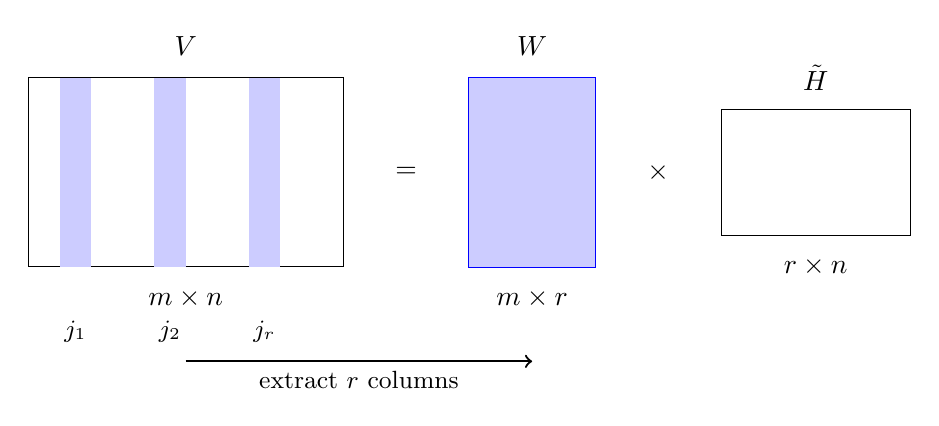
\begin{tikzpicture}[scale=0.8]
    % Matrix V
    \draw (0,0) rectangle (5,3);
    \node at (2.5,3.5) {$V$};
    \node at (2.5,-0.5) {$m \times n$};
    
    % Highlight selected columns
    \fill[blue!20] (0.5,0) rectangle (1,3);
    \fill[blue!20] (2,0) rectangle (2.5,3);
    \fill[blue!20] (3.5,0) rectangle (4,3);
    
    % Column labels
    \node[below] at (0.75,-0.7) {\small $j_1$};
    \node[below] at (2.25,-0.7) {\small $j_2$};
    \node[below] at (3.75,-0.7) {\small $j_r$};
    
    % Equals sign
    \node at (6,1.5) {$=$};
    
    % Matrix W (selected columns of V)
    \draw[thick,blue] (7,0) rectangle (9,3);
    \node at (8,3.5) {$W$};
    \node at (8,-0.5) {$m \times r$};
    \fill[blue!20] (7,0) rectangle (9,3);
    
    % Times sign
    \node at (10,1.5) {$\times$};
    
    % Matrix H-tilde
    \draw (11,0.5) rectangle (14,2.5);
    \node at (12.5,3) {$\tilde{H}$};
    \node at (12.5,0) {$r \times n$};
    
    % Arrow showing extraction
    \draw[->,thick,black] (2.5,-1.5) -- (8,-1.5);
    \node[below] at (5.25,-1.5) {\small extract $r$ columns};
\end{tikzpicture}
\caption{Visualization of separable NMF: the matrix $W$ consists of $r$ selected columns from $V$, indexed by $\{j_1, j_2, \ldots, j_r\}$.}
\label{fig:separable_nmf}
\end{figure}
The separable matrices represent an important class of matrices in applications \cite{arora2012computing}, \cite{gillis2013fast}; for example in text mining \cite{arora2013practical}, 
hyperspectral imaging \cite{boardman1995mapping}, and for some computer vision tasks like background-foreground separation \cite{kumar2015near}.
\par
There are other sufficient conditions that are not included in this thesis, for instance the so called \textit{sufficiently scattered condition} (SCC) is one of them, see \cite{gillis2024checking} for the formulation and an example on how to check it with a global non-convex optimization software; additionally the interested reader may refer to \cite{huang2013non} for a geometrical perspective on uniqueness results.

\section{Geometric Interpretation}\label{Geometric interpretation section}
The aim of this section is to provide a geometric intuition on the NMF problem and provide references to the existent literature that addresses this topic.
This topic is extremely vast therefore in this section only a brief overview is given.
\subsection{Linear dimensionality reduction interpretation}
A way to interpret NMF is that we are seeking a representation of the data points (columns of $V$) as non-negative linear combinations of basis elements (columns of $W$).
That is we wish to find $r$ basis vectors (columns of $W$) such that each data point (column of $V$) can be expressed as a non-negative linear combination of these basis vectors weighted by the coefficients in the corresponding column of $H$.
\begin{equation}
    V[:,j] \approx WH[:,j] = \sum_{k=1}^{r} H[k,j] W[:, k] \quad \forall j = 1, \ldots, n
\end{equation}

\begin{figure}[ht]
\centering
\begin{tikzpicture}[scale=1.3, >=Stealth]
    %  2. Coordinate Definitions
    \coordinate (O) at (0,0);       % Origin
    \coordinate (W1) at (1.8, 2.5); % Vector 1 (Left/Up)
    \coordinate (W2) at (3.0, 1.2); % Vector 2 (Right)
    
    % Define the "Cone" / Subspace
    \coordinate (TopRight) at ($(W1)+(W2)!1.5!(W2)$); % Extrapolation
    \coordinate (FarPoint) at (8, 5.5); % Just a reference
    
    %  3. The Gray Subspace (Cone) 
    % Drawing the filled gray area bounded by W1 and W2
    \fill[red!10] (O) -- (W1) -- (5.5, 4.5) -- (8, 5.2) -- (W2) -- cycle;

    % 4. Basis Vectors 
    \draw[->, thick, red] (O) -- (W1) node[black, midway, left, xshift=-5pt] {\large $W(:,1)$};
    \draw[->, thick, red] (O) -- (W2) node[black, midway, below, yshift=-10pt] {\large $W(:,2)$};

    % 4.1 dashed lines extending the basis vectors
    \draw[dashed, red, thin] (W1) -- (5.5, 4.5);
    \draw[dashed, red, thin] (W2) -- (8, 5.2);

    %  5. Data Points (The 'x' markers) 
    \foreach \p in {
        (1.2, 1.8), (1.5, 2.0), (1.6, 1.2), (2.0, 2.5), (2.2, 1.8),
        (2.5, 3.0), (2.8, 2.2), (3.0, 3.5), (3.2, 1.5), (3.5, 2.8),
        (4.0, 3.2), (4.2, 4.0), (4.5, 3.5), (5.0, 4.2), (5.5, 4.8),
        (1.0, 0.8), (2.5, 1.0), (3.5, 2.0), (4.5, 2.5), (5.8, 3.0),
        (7.0, 5.0), (7.5, 5.3), (6.0, 4.5), (3.0, 4.0), (2.0, 3.5),
        (2.5, 1.5), (3.8, 2.2), (4.8, 3.8), (1.8, 1.0), (0.5, 0.5)
    } {
        \fill[blue] \p circle (2.0pt);
    }

    %  6. Legend (In-plot) 
    \fill[blue] (0, 5.0) circle (2.0pt) node[black, right, xshift=5pt] {\small Data Points (Columns of $V$)};

    %  7. Origin 
    \fill[red] (O) circle (2pt);
    \node[red, anchor=north east, font=\large\bfseries] at (0,0) {0};

    %  8. Mini Coordinate System (Bottom Right Inset) 
    \begin{scope}[shift={(6.5, 0.5)}, scale=0.4]
        \draw[->] (0,0) -- (0,2); % z
        \draw[->] (0,0) -- (1.5,0); % y
        \draw[->] (0,0) -- (-1,-1); % x
    \end{scope}
\end{tikzpicture}
\caption{NMF seeks a low-dimensional non-negative subspace (red area) spanned by basis vectors (red arrows) such that data points (blue dots) lie close to this subspace. Each data point can be approximated as a non-negative linear combination of the basis vectors.}
\label{fig:dimensionality_reduction interpretation}
\end{figure}
In this sense NMF can be thought of as a linear dimensionality reduction technique for matrices of non-negative data.
\subsection{Geometric interpretation with cones}
In linear algebra a convex cone is a subset of a vector space that is closed with respect to the operation of positive scalar multiplication.
\begin{definition}[Convex cone]
A set $C \subseteq \R^m$ is a convex cone if for any $x \in C$ and any non-negative scalars $\alpha \geq 0$ it holds that:
\begin{equation}
    \alpha x \in C
\end{equation}
\end{definition}
Given a matrix $A \in \R^{m \times n}$, the convex cone generated by the columns of $A$ is defined as:
\begin{equation}
    \text{cone}(A) = \{ Ax | x \in \R_+^{n} \}
\end{equation}
\begin{observation}
    $dim(\text{cone}(A)) = rank(A)$
\end{observation}
As seen in \ref{formula for j-th column of V} the $j$-th column of $V$ can be expressed as:
\begin{equation}
    V[:,j] = WH[:,j] \ \forall j = 1, \ldots, n
\end{equation}
This means that each column of $V$ lies in the convex cone generated by the columns of $W$.
In other words:
\begin{equation}
    \text{cone}(V) \subseteq \text{cone}(W)
\end{equation}
% Figure \ref{fig:cone_interpretation} illustrates this concept in two dimensions with $r = 3$.
\par
\begin{figure}[ht]
\centering
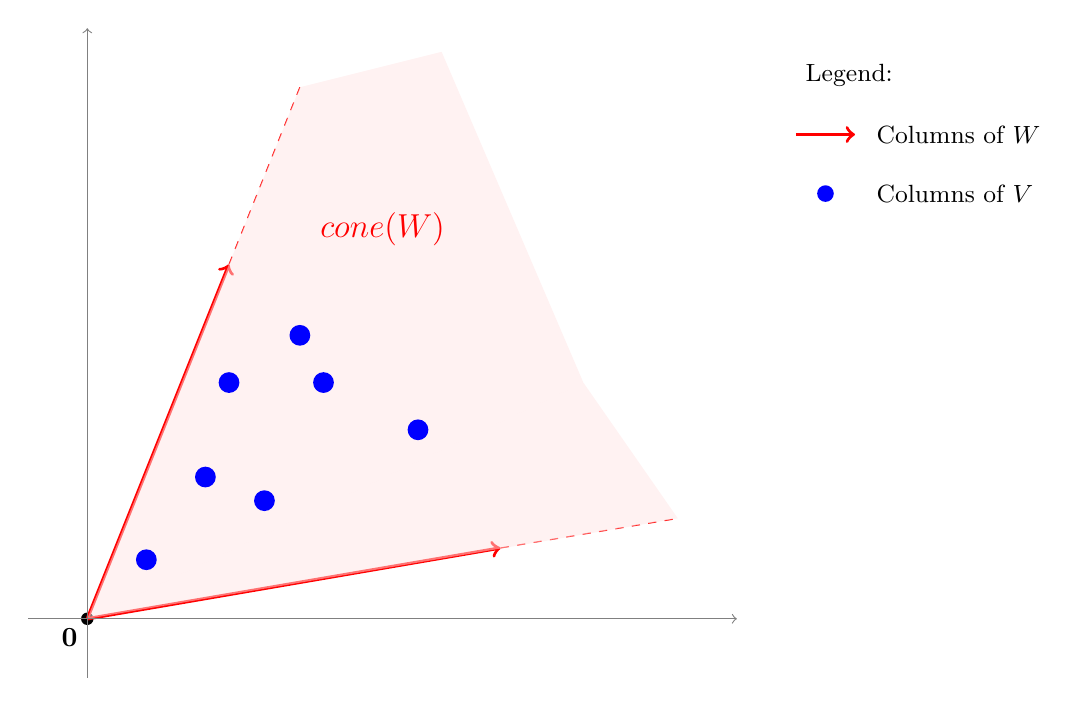
\begin{tikzpicture}[scale=1.5]
    % Origin
    \coordinate (O) at (0,0);
    \fill (O) circle (1.5pt);
    \node[below left] at (O) {$\mathbf{0}$};
    
    % Columns of W (basis vectors)
    %\draw[->,very thick,red] (O) -- (2.5,1.2) coordinate (W1);
    \draw[->,very thick,red] (O) -- (1.2,3) coordinate (W2);
    \draw[->,very thick,red] (O) -- (3.5,0.6) coordinate (W3);
    
    % Cone boundary (dashed lines extending the basis)
    % \draw[dashed,red,thin] (W1) -- (4.2,2);
    \draw[dashed,red,thin] (W2) -- (1.8,4.5);
    \draw[dashed,red,thin] (W3) -- (5,0.85);
    
    % Shaded cone region
    \fill[red!10,opacity=0.5] (O) -- (4.2,2) -- (3,4.8) -- (1.8,4.5) -- cycle;
    \fill[red!10,opacity=0.5] (O) -- (4.2,2) -- (5,0.85) -- cycle;
    
    % Label for cone(W)
    \node[red,font=\large] at (2.5,3.3) {$\text{cone}(W)$};
    
    % Columns of V (data points inside the cone)
        \fill[blue] (0.5,0.5) circle (2.5pt);
        \fill[blue] (1.0,1.2) circle (2.5pt);
        \fill[blue] (1.2,2.0) circle (2.5pt);
        \fill[blue] (2.8,1.6) circle (2.5pt);
        \fill[blue] (1.8,2.4) circle (2.5pt);
        \fill[blue] (1.5,1.0) circle (2.5pt);
        \fill[blue] (2.0,2.0) circle (2.5pt);
    
    % Axes (for reference)
    \draw[->,thin,gray] (-0.5,0) -- (5.5,0);
    \draw[->,thin,gray] (0,-0.5) -- (0,5);
    
    % Legend box
    \begin{scope}[shift={(6,3.5)}]
        % \draw[thick] (-0.3,-0.3) rectangle (2.8,1.5);
        \node[anchor=west] at (0,1.1) {\small Legend:};
        
        \draw[->,very thick,red] (0,0.6) -- (0.5,0.6);
        \node[anchor=west] at (0.6,0.6) {\small Columns of $W$};
        
        \fill[blue] (0.25,0.1) circle (2pt);
        \node[anchor=west] at (0.6,0.1) {\small Columns of $V$};
    \end{scope}
\end{tikzpicture}
\caption{Geometric interpretation: each column of $V$ (blue points) is a non-negative linear combination of the columns of $W$ (red vectors), meaning $V[:,j] = \sum_{k=1}^{r} H[k,j] W[:,k]$. All columns of $V$ lie in the convex cone generated by the columns of $W$.}
\label{fig:cone_interpretation}
\end{figure}
% TODO: add references to literature on geometric interpretation of NMF
Often in the literature the geometric interpretation of NMF is analyzed in terms of nested polytopes.
The reason for this is that because it is easier to visualize and because there is a close connection between the NMF problem in computational geometry known as the and the nested polytope problem (NPP) \cite{shitov2018universalitytheoremnonnegativematrix} \cite{donoho2003does}.
For an overview on the NPP see: \cite{dobbins2019universalitytheoremnestedpolytopes}.
A detailed discussion on the geometric interpretation of NMF can be found in \cite{gillis2020nonnegative} chapter $2.1$.
An example with nested hexagons can be found in \cite{gillis2017introductionnonnegativematrixfactorization}.

\section{Historical origin of NMF}
Even though some early works date back to the 60s in the field of Earth science and remote system sensing \cite{wallace1960analysis}\cite{imbrie1964vector}\cite{craig2002minimum}
the first modern definition of the NMF problem is usually attributed to the work of Paatero and Tapper in 1994 \cite{paatero1994positive} where they defined the so-called Positive Matrix Factorization (PMF) problem, a particular case of NMF where the distance measure used is the least squares one (Frobenius norm).
This early work arose in the field of analytical chemistry and the NMF model as a modern data analysis tool remained relatively unknown until the seminal paper of Lee and Seung in 1999 \cite{Lee1999}.
\par
In their work Lee and Seung introduce the NMF model to the machine learning community and proposed an easy to implement algorithm based on multiplicative updates to find local minima of the NMF optimization problem \ref{NMF optimization problem}.
Their work is especially famous because they  demonstrate an algorithm for non-negative matrix factorization that is able to learn parts of faces, in contrast to other decomposition methods like PCA or SVD that learn holistic features.
Their results are also reproduced in this thesis in section \ref{Example feature extraction NMF} to show a prominent example of NMF's application.




\section{Two applications of NMF}\label{two applications of NMF section}
In this section two applications of NMF are presented: the first one is the well-known example of learning parts of faces introduced by Lee and Seung in \cite{Lee1999},
while the second one is an application of NMF to text mining, in particular to topic modeling.
\subsection{Learning parts of faces} \label{Example feature extraction NMF}
The dataset used in this example is the CBCL face dataset \footnote{See \ref{code documentation appendix} for data availability and details on the code used}.
This dataset has size $361 \times 2429$ where each column represent a $19 \times 19$ gray-scale image of a face.
\begin{figure}[ht]
    \centering
    \includegraphics[width=0.5\textwidth]{Imgs/CBCL_Original.png}
    \caption{Some example images from the CBCL face dataset.}
    \label{fig:CBCL original faces}
\end{figure}
The NMF model is applied to this dataset with a factorization rank of $r = 49$,  the algorithm used is the multiplicative updates with the Kullback-Leibler divergence as distance measure.
After fitting the model we obtain two matrices: $W \in \R_+^{361 \times 49}$ and $H \in \R_+^{49 \times 2429}$.
The non-negativity constraints of the NMF problem \ref{NMF optimization problem} allows one to interpret the columns of $W$ in the same way as the original data, that is each column of $W$ can be reshaped to form a $19 \times 19$ gray-scale image and displayed.
\begin{figure}[ht]
    \centering
    \includegraphics[width=0.75\textwidth]{Imgs/CBCL_colums_of_W.png}
    \caption{Columns of the matrix $W$ reshaped as $19 \times 19$ gray-scale images.}
    \label{fig:CBCL columns of W}
\end{figure}
As can be seen in figure \ref{fig:CBCL columns of W} the pixels of the images formed by the columns of $W$ are active only in certain regions, for example some columns represent eyes, others noses, mouths and so on.
This is the reason why it is said that Non-negative matrix factorization is able to learn a ``part based'' representation of faces.
\par
\begin{figure}[htbp]
    \centering
    \includegraphics[width=0.5\textwidth]{Imgs/Reconstruction_1.png}
    \caption{Example of reconstruction of an image from the CBCL dataset using the NMF model. On the left the original image, on the right the reconstructed one.}
    \label{fig:CBCL reconstructed faces}
\end{figure}
The matrix $H$ contains the coefficients or weights to reconstruct the original images as linear combinations of the parts.\\
The $j$-th column of the original data matrix $V$ can be approximated as:
\begin{equation}
    V[:,j] \approx W H[:,j] = \sum_{k=1}^{r} H[k,j] W[:, k]
\end{equation}
This is a linear combination of the columns of $W$ weighted by the coefficients in the $j$-th column of $H$.
\begin{equation}
    \begin{bmatrix}
        v_{1,j} \\
        v_{2,j} \\
        \vdots \\
        v_{m,j}
    \end{bmatrix} \approx H[1,j]
    \begin{bmatrix}
        w_{1,1} \\
        w_{2,1} \\
        \vdots \\
        w_{m,1}
    \end{bmatrix} + H[2,j]
    \begin{bmatrix}
        w_{1,2} \\
        w_{2,2} \\
        \vdots \\
        w_{m,2}
    \end{bmatrix} + \ldots + H[r,j]
    \begin{bmatrix}
        w_{1,r} \\
        w_{2,r} \\
        \vdots \\
        w_{m,r}
    \end{bmatrix}
\end{equation}
Note that the number of columns of $V$ is equal to the number of columns of $H$. That means that there is a one-to-one correspondence between the columns of $V$ and the columns of $H$ containing the weights to reconstruct each image.
\subsection{Topic modeling}\label{Topic modeling section}
Topic modeling is a technique used in natural language processing and text mining to discover the abstract ``topics'' that occur in a collection of documents.
% It can be though of as a clustering technique where documents are grouped based on the topics they discuss.
\par
The dataset used in this example is the TDT2 corpus, a collection of documents collected in $1998$ \cite{tdt2_corpus} from 6 different sources of american news and only the top (largest) 30 categories are kept. 
The matrix has shape $V \in \R_+^{m \times n}$ where $m = 19528$ is the number of unique words in the vocabulary and $n = 9394$ is the number of documents.
Each column of $V$ represents a document. This is called a word count matrix where each element $V[i,j]$ represents the number of times word $i$ appears in document $j$.
\bigskip    
\begin{longtable}{|c|p{10cm}|}
\caption{Top 10 words extracted by NMF for some of the 30 topics in the TDT2 corpus} \label{tab:nmf_topics} \\
\hline
\textbf{Topic} & \textbf{Top 10 Words} \\ \hline
\endfirsthead

\multicolumn{2}{c}{\tablename\ \thetable\ -- \textit{Continued from previous page}} \\
\hline
\textbf{Topic} & \textbf{Top 10 Words} \\ \hline
\endhead

\hline \multicolumn{2}{r}{\textit{Continued on next page}} \\
\endfoot

\hline
\endlastfoot

1 & iraq, saddam, military, gulf, war, iraqi, arab, hussein, support, attack \\ \hline
2 & cuba, pope, cuban, castro, visit, church, john, paul, popes, havana \\ \hline
3 & tobacco, industry, companies, smoking, bill, legislation, cigarette, congress, senate, settlement \\ \hline
4 & school, students, city, york, police, children, mayor, going, high, news \\ \hline
5 & billion, oil, million, dlrs, prices, percent, tax, economic, budget, exports \\ \hline
6 & lewinsky, jordan, president, tripp, white, lawyers, told, house, relationship, currie \\ \hline
7 & annan, secretary, general, agreement, saddam, sites, kofi, deal, baghdad, inspectors \\ \hline
8 & united, states, american, nations, officials, washington, americans, administration, canada, countries \\ \hline
9 & percent, stock, market, stocks, points, investors, funds, companies, index, fund \\ \hline
10 & israel, israeli, netanyahu, palestinian, peace, palestinians, arafat, bank, talks, west \\ \hline
\end{longtable}

The NMF model is applied to this dataset with a factorization rank of $r = 30$, the algorithm used is the multiplicative updates with the Frobenius norm as distance measure.
After fitting the model we obtain two matrices: $W \in \R_+^{19528 \times 30}$ and $H \in \R_+^{30 \times 9394}$.
The columns of $W$ can be interpreted as topics, where each topic is represented as a distribution over words in the vocabulary.
To extract the top words for each topic we sort the entries of each column of $W$ in descending order and select the top 10 words with the highest weights.
Table \ref{tab:nmf_topics} shows the top 10 words for some of the topics extracted by NMF.
The quality of the clusters can be evaluated by looking at the top words for each topic and checking if they are semantically related, for example in topic 1 we can see that the top words are related to the Iraq war, in topic 2 the top words are related to Cuba and the Pope, in topic 3 the top words are related to the tobacco industry and so on.
\par
The input matrix $V$ is an example of a sparse matrix, because most words do not appear in most documents hence most entries are zero.
In this case the Separability assumption is approximately satisfied because each topic contains some unique words that do not appear in other topics.
This is one of the reasons why NMF works well for topic modeling tasks.
In this case there exists very efficient algorithms to find the NMF solution, see \cite{arora2013practical}.

% filepath: illustrations/document_matrix.tex
\begin{figure}[htbp]
    \centering
    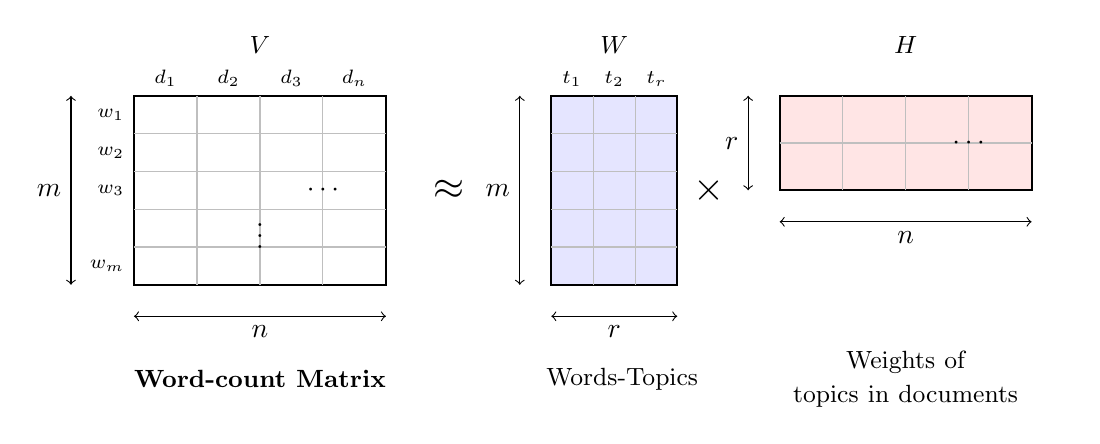
\begin{tikzpicture}[scale=0.8]
        % Document-Term Matrix V
        \draw[thick] (0,0) rectangle (4,3);
        \node at (2,3.8) {\small{\textbf{$V$}}};
        \node at (2,-1.5) {\small{\textbf{Word-count Matrix}}};
        
        % Grid lines for V
        \foreach \x in {1,2,3} {
            \draw[thin, gray!50] (\x,0) -- (\x,3);
        }
        \foreach \y in {0.6,1.2,1.8,2.4} {
            \draw[thin, gray!50] (0,\y) -- (4,\y);
        }
        
        % Labels for documents (columns)
        \node[above] at (0.5,3) {\scriptsize $d_1$};
        \node[above] at (1.5,3) {\scriptsize $d_2$};
        \node[above] at (2.5,3) {\scriptsize $d_3$};
        \node[above] at (3.5,3) {\scriptsize $d_n$};
        
        % Labels for words (rows)
        \node[left] at (0,2.7) {\scriptsize $w_1$};
        \node[left] at (0,2.1) {\scriptsize $w_2$};
        \node[left] at (0,1.5) {\scriptsize $w_3$};
        \node[left] at (0,0.3) {\scriptsize $w_m$};
        
        % Dots to indicate more documents/words
        \node at (3,1.5) {$\cdots$};
        \node at (2,0.9) {$\vdots$};
        
        % Dimensions
        \draw[<->] (-1,0) -- (-1,3);
        \node[left] at (-1,1.5) {$m$};
        \draw[<->] (0,-0.5) -- (4,-0.5);
        \node[below] at (2,-0.5) {$n$};
        
        
        % Equals sign
        \node at (5,1.5) {\Large $\approx$};
        \hspace{0.5 cm}
        % Topic Matrix W
        \draw[thick, fill=blue!10] (6,0) rectangle (8,3);
        \node at (7,3.8) {\small{\textbf{$W$}}};
        
        % Grid for W
        \foreach \x in {6.67,7.33} {
            \draw[thin, gray!50] (\x,0) -- (\x,3);
        }
        \foreach \y in {0.6,1.2,1.8,2.4} {
            \draw[thin, gray!50] (6,\y) -- (8,\y);
        }
        
        % Labels for topics
        \node[above] at (6.33,3) {\scriptsize $t_1$};
        \node[above] at (7,3) {\scriptsize $t_2$};
        \node[above] at (7.67,3) {\scriptsize $t_r$};
        
        % Dimensions for W
        \draw[<->] (5.5,0) -- (5.5,3);
        \node[left] at (5.5,1.5) {$m$};
        \draw[<->] (6,-0.5) -- (8,-0.5);
        \node[below] at (7,-0.5) {$r$};
        
        % Multiplication sign
        \node at (8.5,1.5) {\Large $\times$};
        \hspace{0.5 cm}
        
        % Document-Topic Matrix H
        \draw[thick, fill=red!10] (9,1.5) rectangle (13,3);
        \node at (11,3.8) {\small{\textbf{$H$}}};
        
        % Grid for H
        \foreach \x in {10,11,12} {
            \draw[thin, gray!50] (\x,1.5) -- (\x,3);
        }
        \foreach \y in {2.25} {
            \draw[thin, gray!50] (9,\y) -- (13,\y);
        }
        
        
        % Dots
        \node at (12,2.25) {$\cdots$};
        
        % Dimensions for H
        \draw[<->] (8.5,1.5) -- (8.5,3);
        \node[left] at (8.5,2.25) {$r$};
        \draw[<->] (9,1) -- (13,1);
        \node[below] at (11,1) {$n$};
        
        % Description
        \node[text width=6cm, align=center] at (6.5,-1.5) {\small Words-Topics};
        \node[text width=6cm, align=center] at (11,-1.5) {\small Weights of  \\ topics in documents};
        
    \end{tikzpicture}
    \caption{Non-negative Matrix Factorization of the  word-count matrix $V$ into  the matrices $W$ and $H$.
    Each column of $V$ represents a document, each row represents a word, and each entry is the count of that word in that document.
    }
    \label{fig:document_matrix}
\end{figure}

\section{Summary}

NMF models are able to extract meaningful features and substantial information from non-negative data in many applications. 
The NMF problem is formulated as a constrained optimization problem where the goal is to find two non-negative matrices $W$ and $H$ such that their product approximates the original data matrix $V$.
An NMF model requires to choose a distance measure and a reconstruction rank; NMF model can be extremely versatile and can be adapted to different applications by choosing the appropriate distance measure, possibly with regularization terms, and approximation rank.
To better understand the problem is useful to analyze the exact version of the NMF, known as the exact NMF problem, where the goal is to find two non-negative matrices $W$ and $H$ such that their product is exactly equal to the original data matrix $V$.
In this restricted version of the problem, it naturally arises the definition of Non-negative rank \ref{Non-negative rank section} and the exact-NMF is used for (1) Geometric interpretation of the NMF problem, and (2) to study the computational complexity of the NMF problem, in short the NMF belongs to the class of NP-hard problems. 
Vavasis also showed that that a polynomial-time local search heuristic exists \cite{vavasis2007complexitynonnegativematrixfactorization}. In the next chapter we will see the most important algorithms to undertake the NMF problem, and it will be clear that they come with no optimal guarantees.
